\section{Redegørsel for Mindste Kvadraters Metode}\label{sec:redegorsel}
Antag at du har en række data. Disse data beskriver en sammenhæng mellem tid og distance for en bil. Bilen kører med en konstant hastighed. Du har nu brug for at finde ud af hvor langt bilen har kørt efter 10 sekunder. Dette ingår dog ikke i datasættet. For at finde denne information kunne man fx. opstille en funktion der beskriver denne sammenhæng. For at beskrive denne sammenhæng, kunne Mindste Kvadraters Metode anvendes. Mindste Kvadraters Metode anvendes ofte til at beskrive en ret linje. (\begin{math}y = ax + b\end{math}) En ret linje kan beskrives på mange måder. Dog vil der kun være en linje der beskriver datasætte bedst. For at finde frem til det krever det, at der fordybes i funktioner af to variable, samt hvordan de afledes.

% Redegør for matematikken bag Mindste Kvadraters Metode (Få sammen sat afsnitet funktioner med to variable og Mindste Kvadraters Metode på en god måde)

\subsection{Funktioner med to variable?}\label{sec:FunktionerMedToVariable}
Du har måske stiftet bekendskab med funktioner af en variabel. Disse funktioner er ofte skrevet som \begin{math}f(x) = x^2\end{math}. Her ønsker man at finde en værdien $f(x)$ for en givet $x$ værdi. Her giver man altså en værdi og får en værdi tilbage. Men hvad nu hvis du skal beskrive en sammmenhæng, der er afhængig af to variabler? Her kommer funktioner med to variabler ind i billedet. Når der arbejdes med funktioner af en variabel forgår dette i et koordinatsystem med en x-akse og en y-akse. Altså et todimensionelt koordinatsystem. For at kunne afbillede funktioner af to variable, arbejdes der ikke længere i et koordinatsystem med todimensionelt, men i et tredimensionelt koordinatsystem. Her er der en x-akse, en y-akse og en z-akse. Den nye akse (z-aksen) står vinkelret på de to andre akser (\cite[246-248]{funktionrAfToVariable}). For at bedre forstå hvordan det tredimensionelle  koorinatsystem hænger sammen kan man tænke på det som en kasse. Hvor x-aksen er længden, y-aksen er bredden og z-aksen er højden. Når der arbejdes med funktioner af to variable vil den typiske notation se således ud: $f(x,y)$ her er både $x$ og $y$ variabler. Disse to variable kan bruges til at beskrive et punkt i det tredimensionelle koordinatsystem. Dette skyldes at $z = f(x,y)$ Et konkret eksempel kunne være et vejrkort. Her er temparaturen afhængig af to variable. Her angiver $x$ og $y$ en lokation og $z$ angiver temparaturen. På den måde afgænger temparaturen af to variable, det geografiske punkt som beskrives $(x,y)$.\\

% Hvad mangler der at blive redegjort for i dette afsnit? (Hvordan kobler vi dette sammen med Mindste Kvadraters Metode? Grafisk afblidning af funktion. Saddelpunkt?)

\subsubsection{Partielt differentiation}\label{sec:PartieltDifferentiation}
For at finde hældningen af tangenten til en funktion af to variable, skal man gå igennem en lidt længere proces end ved funktioner af en variabel. For at finde hældningen af tangenten til funktionen af en variabel, diffrencere man med hensyn til $x$. Et eksempel kunne være $f(x) = x^2$ her er $f'(x) = 2x$. Dette skyldes følgende regneregl: $a \cdot x^n$ bliver til $a \cdot n \cdot x^{n-1}$. Det er dog ikke lige så simpelt at finde hældningen af tangenten, til en funktion af to variable. Her skal man benytte sig af en metode kaldt: Partial differentiation. Ved partial differentiation, tages der fat i en variabel ad gangen. Partial betyder delvis. Grunden til at dette ord anvendes er da man diffrencere mht. $x$ og $y$ i hver deres led (\cite[4]{Larsen2016}). For lige at tage et eksempel så antages det at en funktion hedder: 
\begin{equation}f(x,y) = x^2 + 3y^2\end{equation}
Opgaven er her at finde den partial aflededet funktionen $f'(x,y)$. For at finde den partielle afledede for funktionen $f(x,y)$ startes der med at sætte en af variablerne til en konstant. I dette tilfælde sættes $y$ til en konstant. Dette gøres for at man kan nøjes med at diffrencere mht. $x$. Når der diffrenceres med en funktion af en variabel, agives dette sådan: \begin{equation}\frac{d f(x)}{d x}\end{equation} Sådan er det dog ikke ved partial differentiation. Her angives det sådan: \begin{equation}\frac{\partial f(x,y)}{\partial x}\end{equation} Dette er for at vise, at der diffrenceres partielt. Ret simpelt så definere det bløde d ($\partial$) bare at der diffrenceres partielt. Hvis der igen tages udgangspunkt i eksempelet fra før, hvor $f(x,y) = x^2 + 3y^2$. Så ville den partielle afledede af $f(x,y)$ med hensyn til $x$ være: \begin{equation}\frac{\partial f(x,y)}{\partial x} = 2x\end{equation}
Dette skyldes at $y$ er en konstant og derfor ikke indgår i diffrencering. Der skal nu findes den partielle afledede af $f(x,y)$ med hensyn til $y$. Dette gøres ved at sætte $x$ til en konstant. Dette vil give følgende resultat: \begin{equation}\frac{\partial f(x,y)}{\partial y} = 6y\end{equation} Den partielt aflededet må derfor være $f'(x,y) = 2x + 6y$. Dette er hældningen af tangenten til funktionen $f(x,y)$ i punktet $(x,y)$ (\cite{Carstensen2024}).

\subsection{Sådan finder du frem til den bedste funktion}
For at forstå hvordan der findes frem til den bedste funktion. Skal der findes frem til en metode hvorpå det er muligt at beskrive hvor god en funktion er.
Den umilbare bedste måde at beskrive linjen på er ved at kigge på afstanden fra punkt til linje. Dette kan gøres på flere måder. Afstanden kunne være den vinkelrette afstand fra linjen ned til punktet, dette er dog ret svært at regne med, og i stedet findes den lodrette afstand fra punkt til linje.Dette gøres ved at finde forsællen i y-værdierne.
\begin{wrapfigure}{r}{0.5\textwidth}
    \centering
    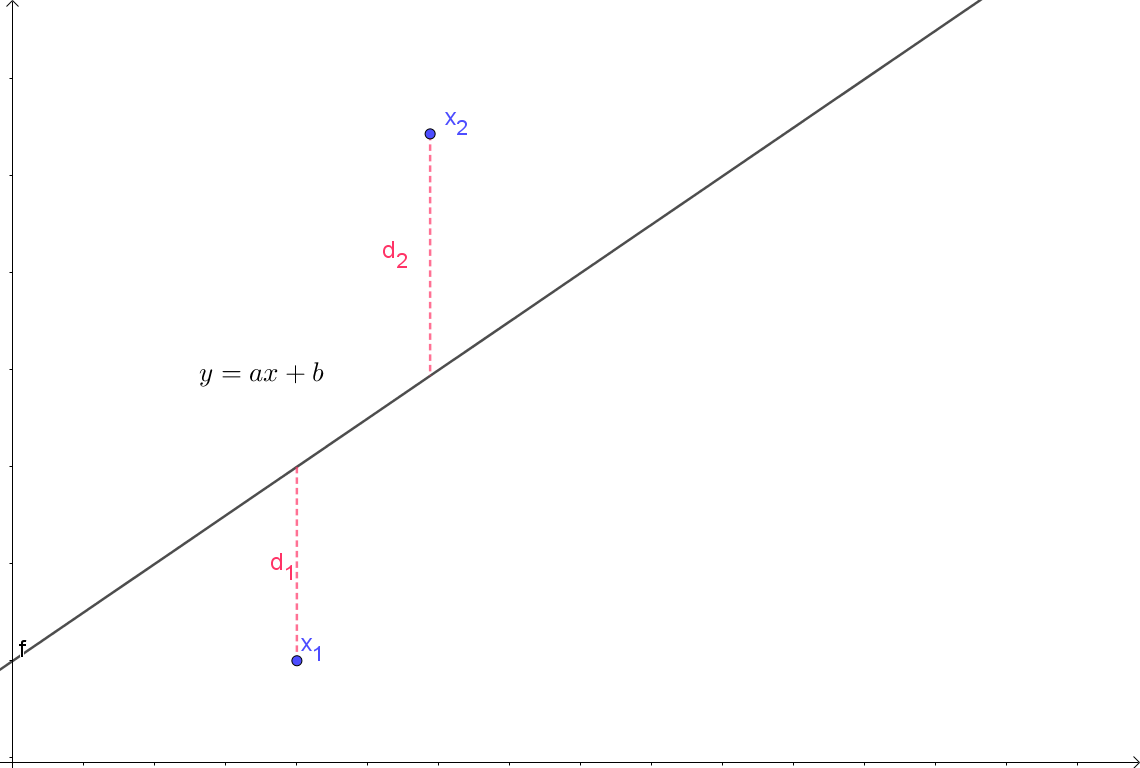
\includegraphics[width=0.5\textwidth]{figures/afstand.png}
    \caption{Afstand fra punkt til linje}
    \label{fig:afstandFraLinjeTilPunkt}
\end{wrapfigure}   
Dette skaber dog en ting man skal være opmærksom på. Nemlig at der kan være punkter over og under linjen. For at undgå at afstanden udligner hindanden opløftes afstanden derfor i anden 
(\cite[2]{ForberedelsessetMaj2013}). Se figur \ref{fig:afstandFraLinjeTilPunkt} for grafisk ilustration 
Da der nu er styr på hvordan afstanden fra punkt til linje findes. Der skal nu findes en metode hvorpå det er muligt at beskrive afstanden ift linjen. Hvis der startes med at tage udgangspunkt i et punkt. Punktet kunne hede hvad somhelst og dog hedder linjen: $y = a \cdot x + b$. Så må afstanden i y-værdien kunne beskrives som \begin{equation}\label{eq:distance}
    d_n = a \cdot x_n + b - y_n
\end{equation} grunden til at $y_n$ fratrækkes, er at y-værdien for linjen ved $x_n$ ville være $y =a \cdot x + b$. På den måde kan afstanden altså bestemmes. Afstanden har på den måde nu dannet en ligning med to ubekendt der beskriver arealet af en kvadrat. Da det jo som nævnt før opløftes i anden så må det være det samme som at regne arealet af en kvadrat (\cite{Bentzen2014}). Nu begynder navnte Mindste Kvadraters Metode lige så stille at give mening. Da målet er at finde den linje hvor Kvadraternes areal er mindst. For at regne distance fra punkt til linje for alle punkter anvendes formlen: \ref{eq:distance}, dette skal gøres for alle punkter. Deres fælles areal kan derfor beskrives som følgende:
\begin{equation}A = \sum_{n=1}^n (a \cdot x_n + b - y_n)^2\end{equation}
Resultat af denne udregning kunne omskrives til en funktion af to variable, hvor $a$ og $b$ er de ubekendte. Der hvor arealerne er mindst må de to ubekendte danne den best mulige linje. Dette ville kunne ses som et ekstrema, på funktionen af variavble $a$ og $b$. Dette ekstrema findes ved at lave partial diffrencering (Se afsnit \ref{sec:PartieltDifferentiation}) af funktionen med hensyn til $a$ og $b$ og til sidst sætte differentialkvotienterne til 0. Dette skyldes at når hældningen af tangenten er nul så vil der være enten et toppunkt eller minimumspunkt. Der vil nu være dannet to ligninger med hvor de ubekendte vil være hhv $a$ og $b$ Disse to ligninger kan løses og dermed findes den bedste linje. (\cite{webmatematikMindsteKvadratersMetode})


\section{Praktisk anvendelse af Mindste Kvadraters Metode}\label{sec:udregning}
Med baggrund i afsnit \ref{sec:redegorsel} om redegørsel for Mindste Kvadraters. Kan metoden nu anvendes på datasættet om bilen der kører med konstant hastighed. Datasættet viser sammenhængen mellem tid og den tilbagelagte distance for bilen:
\begin{table}[h!]
    \centering
    \begin{tabular}{|c|c|} \hline
        $Tid [s]$ & $Distance [m]$ \\ \hline
        $1$ & $6$ \\ 
        $5$ & $6$ \\
        $6$ & $12$ \\
        $10$ & $10$ \\ \hline
    \end{tabular}
    \caption{Sammenhæng mellem tid og distance.}
\end{table}\\
Der skal nu findes frem til den funktion der vil beskrive sammenhængen bedst. Først sættes der en lining op der beskriver alle punkternes kvadrater.
\begin{equation*}
    A = (a \cdot 1 + b - 6)^2 + (a \cdot 5 + b - 6)^2 + (a \cdot 6 + b - 12)^2 + (a \cdot 10 + b - 10)^2
\end{equation*}
Dette kan ved hjælp af kvadrat sætningen \begin{math}(a+b)^2 = a^2 + b^2 - 2ab\end{math} omskrives til:
\begin{equation*}
    4b^2+44ab-68b+162a^2-416a+316
\end{equation*}
Dette bliver nu en funktion af to variable, hvor $a$ og $b$ er de ubekendte.
\begin{equation*}
    f(a,b) = 4b^2+44ab-68b+162a^2-416a+316
\end{equation*}
For at finde ekstrema for funktionen $f(a,b)$ skal der partielt aflededes med hensyn til $a$ og $b$.
\begin{equation*}
    \frac{\partial f(a,b)}{\partial a} = 324a - 416
\end{equation*}
\begin{equation*}
    \frac{\partial f(a,b)}{\partial b} = 8b - 68
\end{equation*}
Differentialkvotienterne sættes nu til 0.
\begin{equation*}
    324a - 416 = 0
\end{equation*}

\begin{equation*}
    8b - 68 = 0
\end{equation*}
% DETTE ER TOTALT FORKERT





% Vis hvordan Mindste Kvadraters Metode kan anvendes på et selvvalgt datasæt (Husk en fortolkning af resultaterne)


\section{Implementering af Mindste Kvadraters Metode}
% Anvend pseudokode til at vise hvordan Mindste Kvadraters Metode kan implementeres


\subsection{Program Design}
% Forklar hvilke overvejelser der er gjort i forhold til program design, sprogvalg, biblioteker, etc. Teorisk baggrund!!!

\subsection{Program redegørsel}
% Redegør for programmet og dets funktioner (Husk at inkludere kodeeksempler)

\section{Fordele og Begrænsninger}
%Her analyseres metoden på et bredere niveau ved at vurdere dens styrker og svagheder i en programmeringssammenhæng.

\section{Diskussion af Kodningsmetoder}
% While loops, for loops, rekursive funktioner, ect.

\section{Konklusion}

\section{Perspektivering}
